\chapter{File storage and backup}
\label{chap:storage}

\section{SFTP-only access model}

Storage-Service stores the users' backups and is the only component the client talks to
directly after authentication.
Indeed, once authenticated, the user becomes able to reach it on the private network
and is therefore ready to manage their backups.

Before transmitting them, however, the user's client, through Restic \cite{restic-github}, deduplicates, compresses, and
encrypts the user's backups. Storage-Service therefore receives a sequence of encrypted blocks that it is not
able to decrypt.
When initializing the Restic repository, the client draws 32 bytes from \texttt{crypto/rand},
encodes them in base64 and uses them as the repository password \cite{ramusb-code-reposecret}.
From that password Restic derives the key that opens the file in which it keeps the actual encryption key,
generated at random when the repository is created \cite{restic-design}: it is the latter that protects the blocks.

This approach was designed to prevent the user from choosing a weak
password. The client saves the repository password on the user's device, with the same
permissions as the SSH private key. Its secrecy, like the responsibility of copying the keys to
a safe place, is left to the user. Should even a single one of the
credentials be lost, the user would have no way to access the content of their backups.

The fact that the users' data is encrypted, however, does not mean that it should be reachable by
anyone.
The only way to reach the blocks is in fact an authenticated SFTP session, inside the private
mesh network. On that session, the only possible operation is transferring files, and the only credential
accepted is the SSH key \cite{openssh-sshd-config}.

Left out are the other ways of authenticating and the other uses that SSH normally allows, such as executing a command,
opening a shell, or using the connection as a relay to reach other machines.

Moreover, only the accounts created by the service can log in, because the server accepts only
usernames of the form \texttt{user*} and root access is explicitly disabled.

OpenSSH's default list of cryptographic algorithms \cite{openssh-sshd-config} is deliberately broad
to guarantee compatibility with clients that do not support the modern and more robust algorithms, but here that
compatibility is not needed, and only risks weakening the system; therefore, the cryptographic
algorithms are also listed by hand \cite{ramusb-code-sshd-config}.

\section{Isolation and dynamic chroot}
\label{sec:isolamento}

Isolation between users rests on an operating system mechanism called chroot, which
confines a process inside a subdirectory: from that moment on that directory is, for the process, the
root of the filesystem, and outside of it there is no longer any path that the process can
name.

At registration, Storage-Service prepares for the new user the POSIX account that will inhabit that
space. The account has no traditional home directory and its shell is \texttt{/usr/sbin/nologin},
a program that merely refuses access.

For every POSIX user whose name matches \texttt{user*}, the rules
specified in \autoref{lst:sshd-match} are also applied.

\Needspace{10\baselineskip}
\begin{lstlisting}[language=sshdconfig, caption={The two per-user directives, from
\texttt{sshd\_config} \cite{ramusb-code-sshd-config}, with added comments.},
label={lst:sshd-match}]
Match User user*
    ChrootDirectory /storage/%u   # confines the session to the user's subtree
    ForceCommand internal-sftp    # enforces SFTP in place of the command requested by the client
\end{lstlisting}

Alongside the account, the directory structure illustrated in
\autoref{fig:filesystem-storage} is created. The root of the confinement belongs to root, while the
\texttt{data} subdirectory belongs to the user and is the only place where they can write.
Ownership by root is a requirement of the SSH server, which
refuses to confine a session in a directory writable by anyone else.

The result is that a connected user sees as the root of their filesystem the directory that
belongs to them, and the other users' directories are neither reachable nor listable in any way.

Normally an SSH server looks for the keys that authorize a connection in a file inside the user's
home, where the keys accepted for that account are listed. Here that file is not
consulted.
In its place, at every connection attempt, the server runs a dedicated binary, passing it the
username being presented. The binary runs under a system identity that has no other
duties on the machine and asks Database-Vault for that user's current public key over an
mTLS channel.

Whatever goes wrong produces the same outcome: the binary exits without printing anything
\cite{ramusb-code-authkeys-cmd}. The server receives an empty list of keys and denies the connection,
following the fail-secure principle \cite{owasp-fail-securely}.
There is no other place outside Database-Vault in which the SSH public keys are stored,
so a malfunction in Database-Vault prevents users from starting SFTP sessions.

\section{Backup and restore}
\label{sec:backup-restore}

The backup takes place entirely on the user's device. The client invokes Restic, indicating as the
repository the writable subdirectory inside the user's own confined space, reached via SFTP, and
requires it to authenticate with the private key generated at registration
\cite{ramusb-code-restic-sftp}, which has never left the machine and which no component of the
system has ever seen.

The path given for the repository is already relative to the root of the confinement.

The client resolves Storage-Service through MagicDNS on the mesh network,
and the resolution succeeds only as long as the temporary grant given by the last login is active:
once that has expired, the user's node no longer sees the service and the connection does not even start.
\autoref{chap:rete} describes how that grant is given and revoked.

\autoref{fig:uc03} summarizes the sequence, from the SFTP connection to the written data.

\begin{figure}[H]
    \centering
    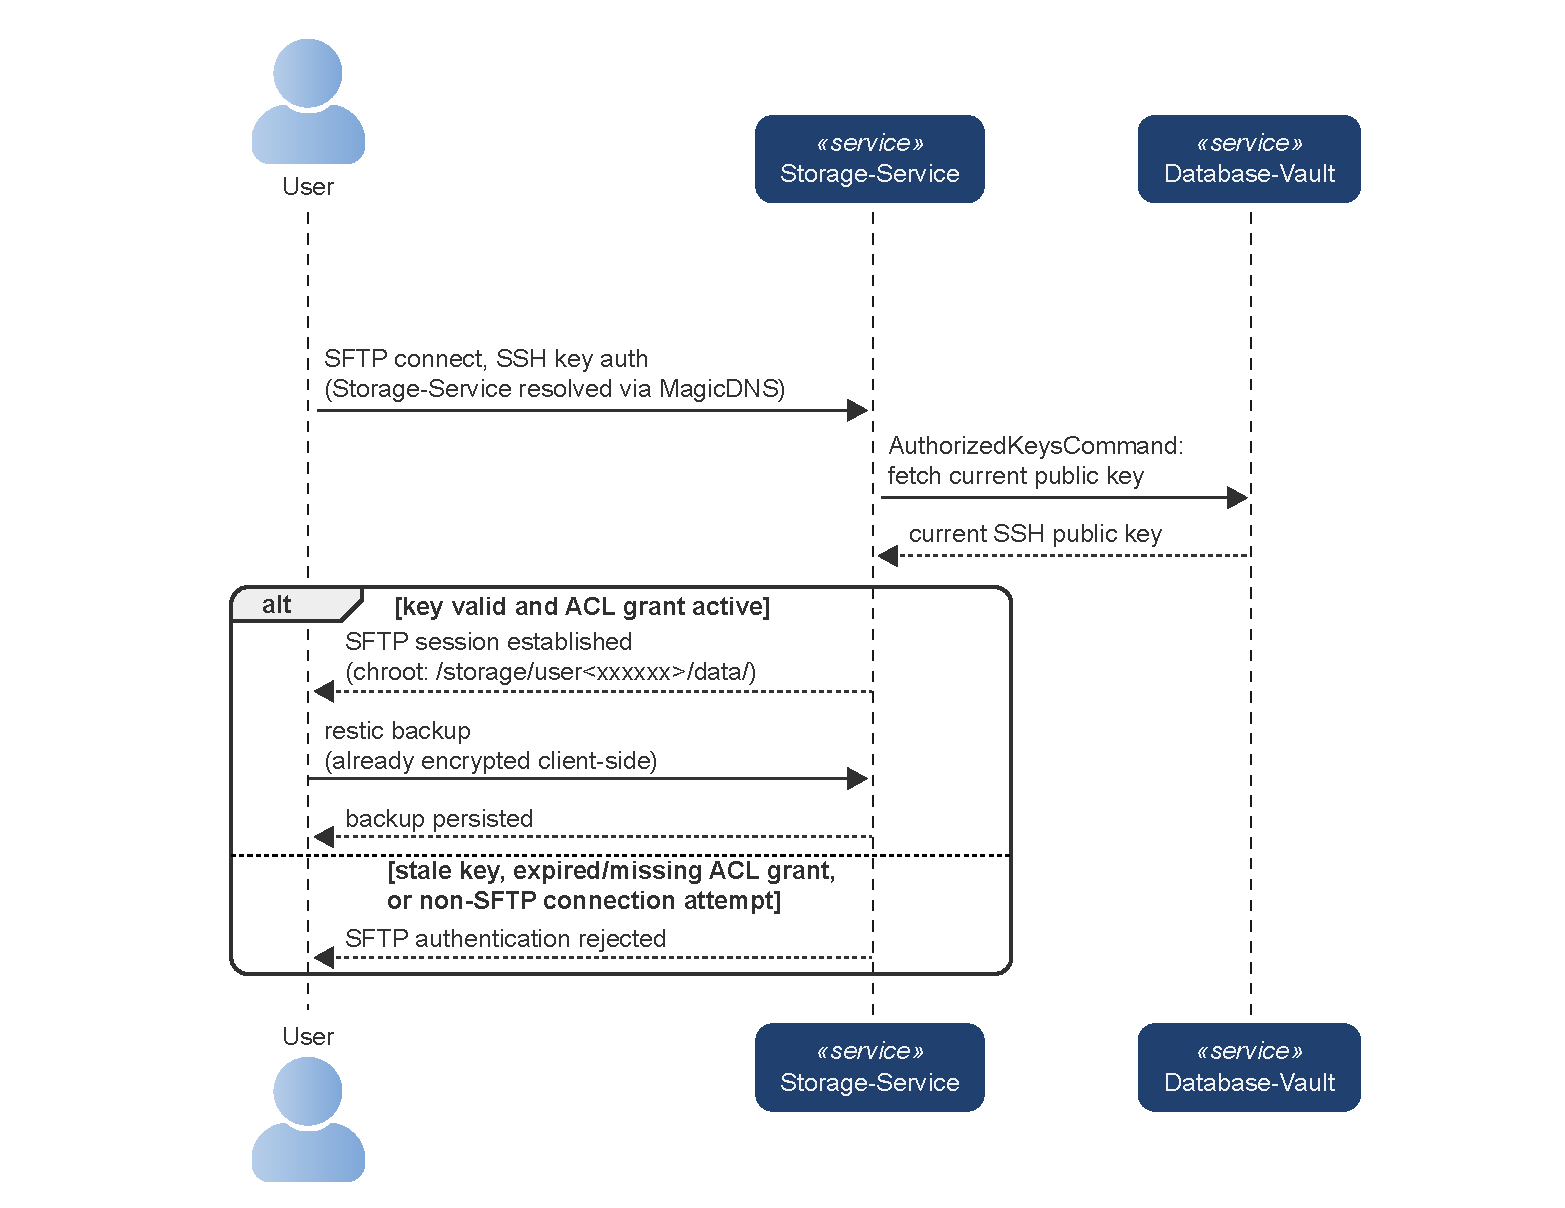
\includegraphics[width=0.8\textwidth]{figures/05-usecases-sequence-uc03-backup.pdf}
    \caption{Sequence for backing up a file (UC-03).}
    \label{fig:uc03}
\end{figure}

Restore follows the same path as backup; the only difference is the command issued to
Restic, which downloads the requested blocks and decrypts them on the user's device.
